\chapter{Composition of Fault Forests}
\label{chap:compFF}
Proving that the system operates within some level of safety when failures are present is an important aspect of critical systems development and falls under the discipline of safety analysis. Safety analysis produces various safety related artifacts that are used during development and certification of critical systems~\cite{SAE:ARP4754A}. Examples include {\em minimal cut sets} -- each set represents the minimal set of faults that must all occur in order to violate a safety property and {\em fault trees} -- the evaluation that determines all credible failure combinations which could cause an undesired top level hazard event. The fault tree can be transformed to an equivalent Boolean formula whose literals appear in the minimal cut sets. Since the introduction of minimal cut sets in the field of safety analysis, much research has been performed to address the generation of these sets and associated formulae~\cite{vesely1981fault,fta:survey,historyFTA}. As critical systems get larger, more minimal cut sets are possible with increasing cardinality. In recent years, symbolic model checking has been used to address scaling the analysis of systems with millions of minimal cut sets~\cite{bieber2002combination,schafer2003combining,symbFTA}. 

The state space explosion is a challenge when performing formal verification on industrial sized systems. Compositional reasoning takes advantage of the hierarchical organizaton of a system model as verification is performed. A compositional approach verifies each layer of the system hierarchy in isolation and allows global properties to be inferred about the entire system~\cite{berezin1997compositional}. The {\em assume-guarantee} paradigm is commonly used in compositional reasoning. If the assumed behavior of the components is true, then the guarantee will hold~\cite{cofer2012compositional}.

In Chapter~\ref{chap:faultModeling}, we described how to perform behavioral fault analysis using the safety annex. This approach allows for either monolithic or compositional analysis. In monolithic analysis, the model is flattened and all component contracts are used in the proof of a safety property. Any failures that occur at the leaf level will be reflected at the top of the system hierarchy. In compositional fault analysis, this is not the case. Compositional analysis is performed from the top down and progresses per layer of the system architecture. An active fault at a leaf level may violate guarantees at its parent level and this will be seen in the fault analysis for that layer. But if that parent level guarantee is necessary for proving a safety property of the system, no indication of this can be shown. We wish to reflect errors in leaf level components at the top of the hierarchy in a compositional manner. 

Using an assume-guarantee reasoning framework, we extend the definition of the nomimal transition system to allow for the possibility of unconstrained output corresponding to violated guarantees. We use this idea to reason about all possible violations of a safety property per layer of analysis and then compose the results. The formalization defines a sound approach to the composition of the Boolean formulae that describe component fault trees.

After we provide the formalization, we describe the implementation in the OSATE tool for the Architecture and Analysis and Design Lanugage (AADL)~\cite{FeilerModelBasedEngineering2012}. AADL has two annexes that are of interest to us: the Assume-Guarantee Reasoning Environment (AGREE)~\cite{cofer2012compositional} and the safety annex~\cite{stewart2020safety}. AGREE provides the assume-guarantee reasoning required fornominal model analysis, and the safety annex allows us to define faults on component outputs. For the implementation of this compositional approach, we look to recent work in formal verification. Ghassabani et al.~developed an algorithm that traces a safety property to a minimal set of model elements necessary for proof; this is called the \textit{all minimal inductive validity core} algorithm (\aivcalg)~\cite{GhassabaniGW16,Ghassabani2017EfficientGO}. Inductive validity cores produce the minimal sets of model elements necessary to prove a property. Each set contains the behavioral contracts -- the assumptions and guarantees of components -- used in a proof. We collect all MIVCs per layer to generate the minimal cut sets and thus the fault trees to be composed.


This chapter presents a compositional approach to generating fault forests (sets of fault trees) and associated minimal cut sets, allowing us to reason uniformly about faults in hardware and software and their impact on system properties. 

\section{Running Example}
\label{sec:example}
In a typical Pressurized Water Reactor (PWR), the core inside of the reactor vessel produces heat. Pressurized water in the primary coolant loop carries the heat to the steam generator. Within the steam generator, heat from the primary coolant loop vaporizes the water in a secondary loop, producing steam. The steamline directs the steam to the main turbine causing it to turn the turbine generator, which in turn produces electricity. There are a few important factors that must be considered during safety assessment and system design. An unsafe climb in temperature can cause high pressure and hence pipe rupture, and high levels of radiation could indicate a leak of primary coolant~\cite{PWR}. 

\begin{figure}[h!]
	%\vspace{-2em}
	\begin{center}
		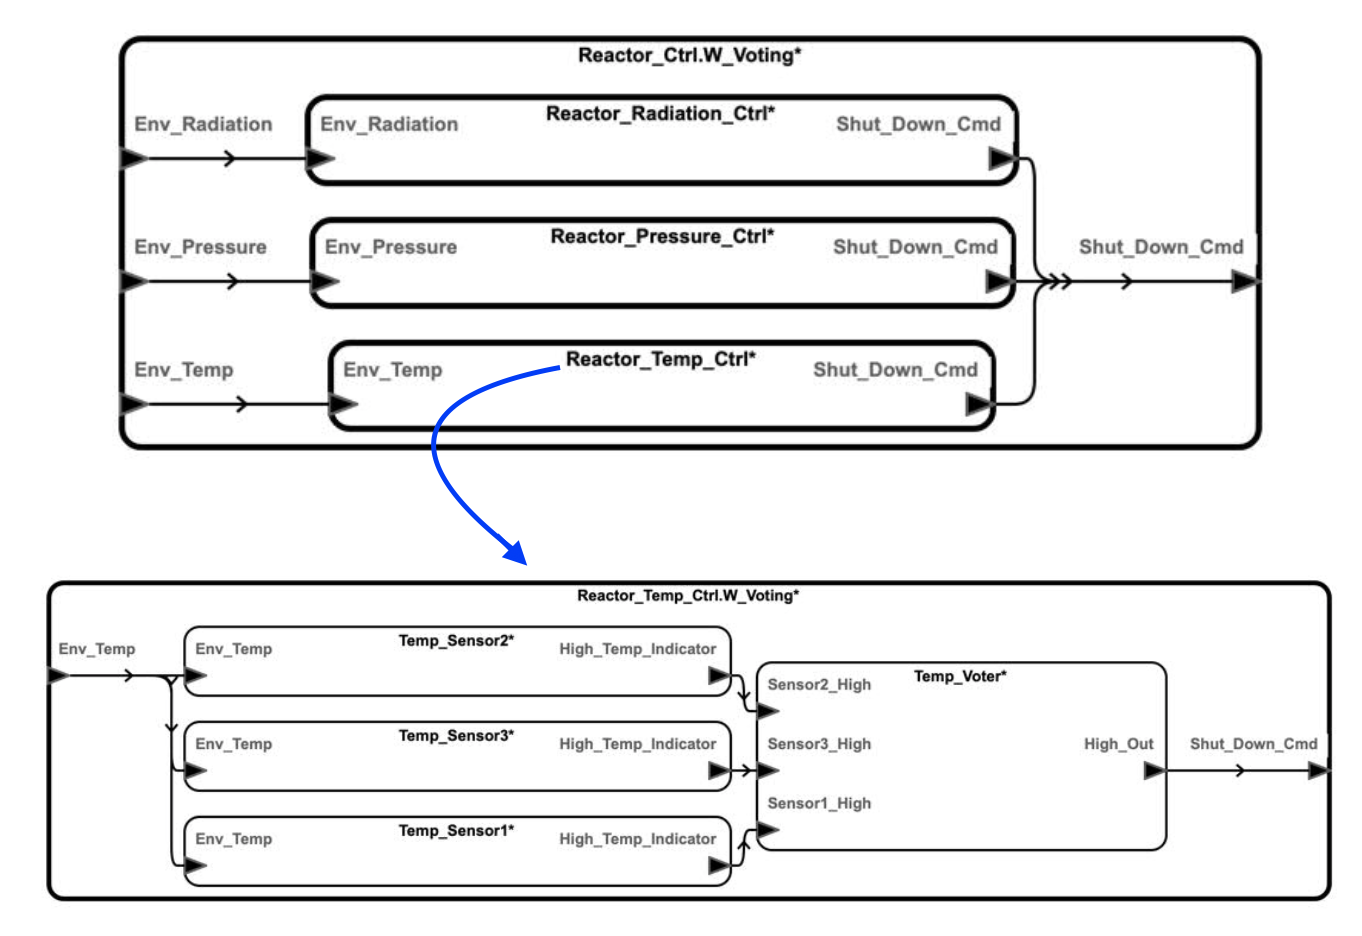
\includegraphics[width=0.8\textwidth]{images/sensorSysAADL.png}
	\end{center}
	%\vspace{-2em}
	\caption{PWR Sensor System}
	\label{fig:sensorSys}
	%\vspace{-2em}
\end{figure}

The following sensor system can be thought of as a subsystem within a PWR that monitors these factors. A diagram of the model is shown in Figure~\ref{fig:sensorSys} and represents a much simplified version of a safety critical system. The temperature subsystem details are shown at the bottom of Figure~\ref{fig:sensorSys}; each of the subsystems have a similar architecture.

Each subsystem contain three sensors that monitor pressure, temperature, and radiation. If any of these conditions are too high, a shut down command is sent from the sensor subsystem to the parent component. 

The temperature, pressure, and radiation sensor subsystems each contain three associated sensors for redundancy. Each sensor reports the associated environmental condition to a majority voter component. If the majority of the sensors reports high, a shut down command is sent to the subsystem. If any subsystem reports a shut down command, the top level system will shut down. Pressure, radiation, and temperature all have associated thresholds for high values which we refer to as $T_p$, $T_r$, and $T_t$ respectively. The safety property $P$ of interest in this system is: \emph{shut down when and only when we should} and is reflected by the shut down command at the top level where $T_t$, $T_p$, and $T_r$ are the thresholds associated with temperature, pressure, and radiation respectively:

\begin{equation*}
shutdown =  (Env\_Temp > T_t)  \lor  (Env\_Pressure > T_p) \lor (Env\_Radiation > T_r)
\end{equation*}

For reference throughout this paper, we provide Figure~\ref{fig:sensorSysContracts} which shows the guarantees and faults of interest for this running example. 

\begin{figure}[h!]
	%\vspace{-6em}
	\begin{center}
		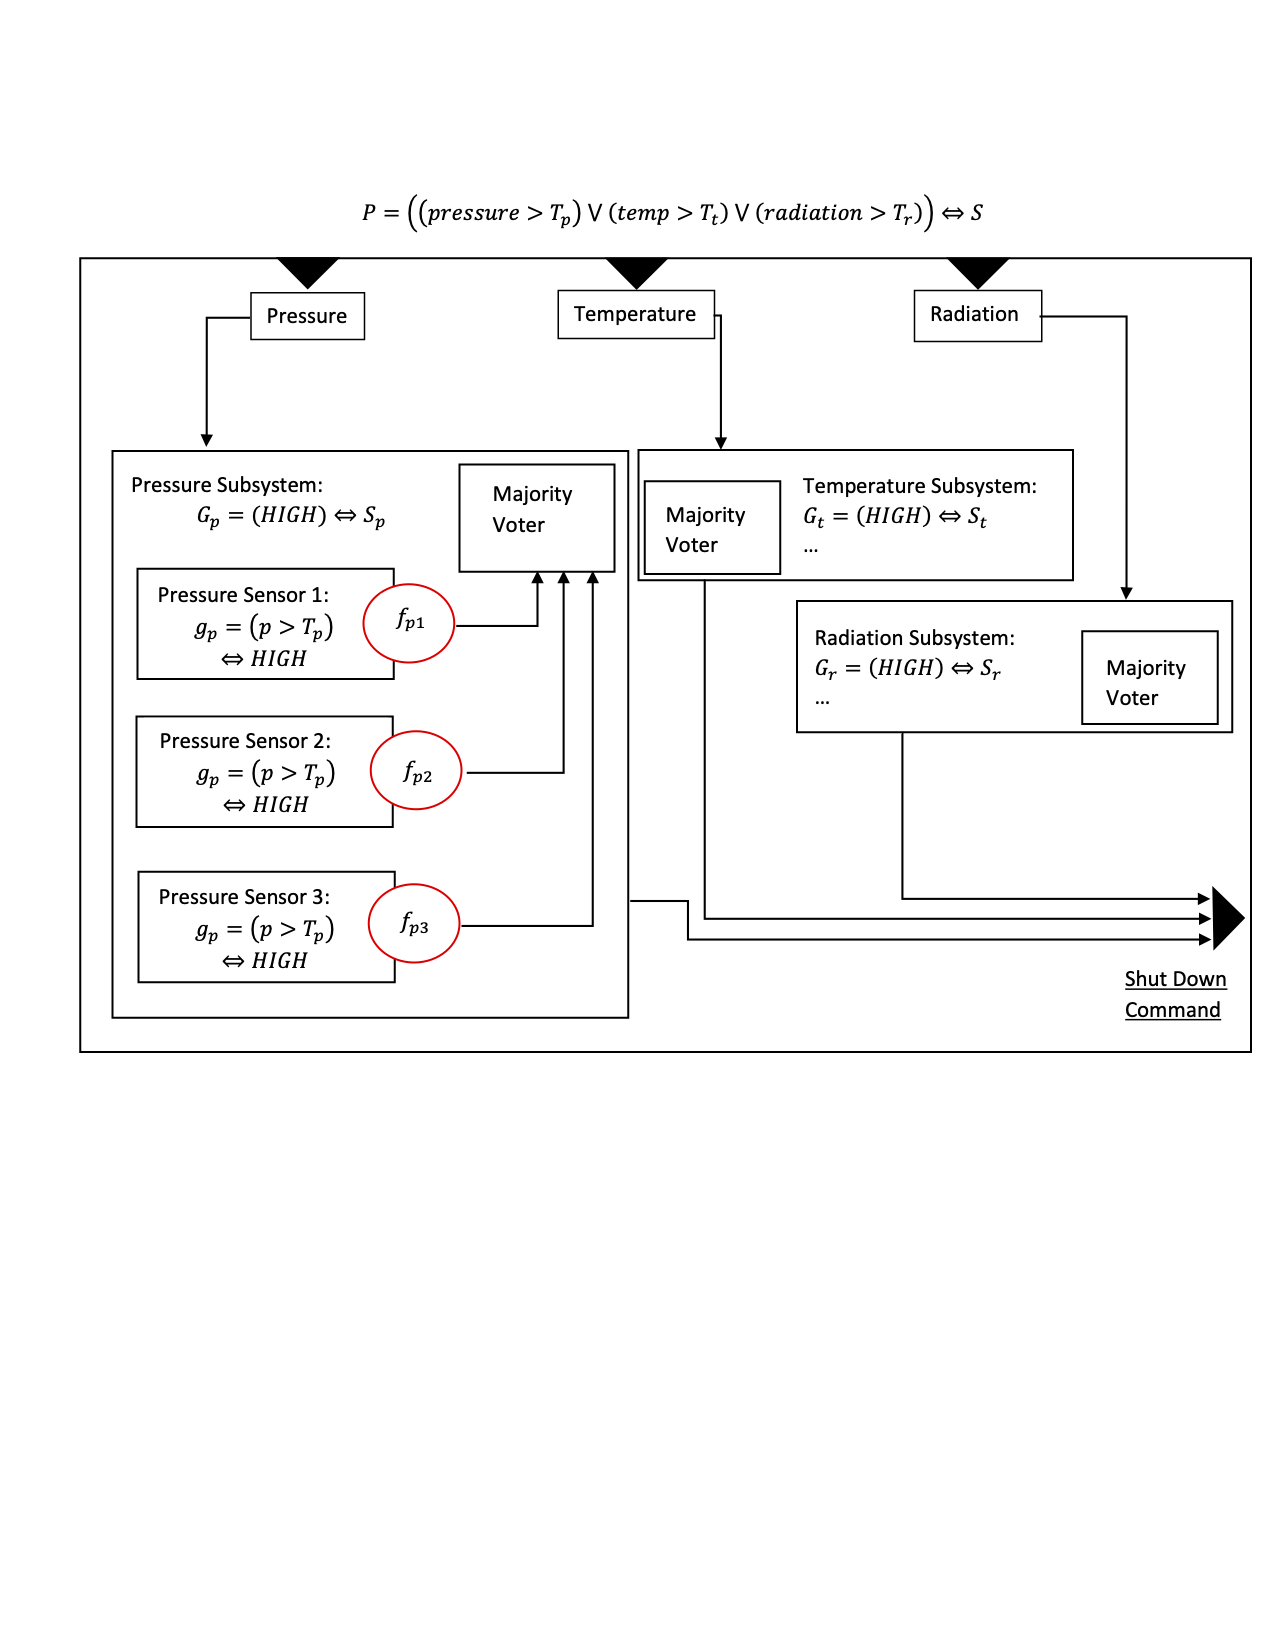
\includegraphics[width=1.0\textwidth]{images/PWRFigureContracts.png}
	\end{center}
	%\vspace{-4em}
	\caption{Sensor System Nominal and Fault Model Details}
	\label{fig:sensorSysContracts}
	%\vspace{-2em}
\end{figure}

The top level shut down command is given as $S$ and each sensor subsystem provides their own shutdown command, $S_p$ for example.  We do not show all guarantees and assumptions that are in the model, but only the ones of interest for the illustration. Initially, assume that the faulty behavior is simply unconstrained output, or the possible violation of a guarantee. This is equivalent to the removal of the guarantee from the model. For our purposes in the next section, this situation is what we want to explore. When we describe the implementaton in Section~\ref{sec:impl}, we define more concrete failure scenarios.

\begin{comment}
\subsection{PWR Fault Model}
The faults that are of interest in this example system are any one of the sensors failing high or low. If sensors report high and a shut down command is sent, we shut down when we should not. On the other hand, if sensors report low when it should be high, a shut down command is not sent and we do not shut down when we should. From the perspective of safety, a false report of low temperature is the main concern. For simplification in this paper, we focus on the failures when sensors report low when they should not.

A fault is defined for each sensor in the system using the safety annex. An example of a temperature sensor fault stuck at high is shown in Figure~\ref{fig:tempSensorFault}.

\begin{figure*}[h!]
	%\vspace{-2em}
	\begin{center}
		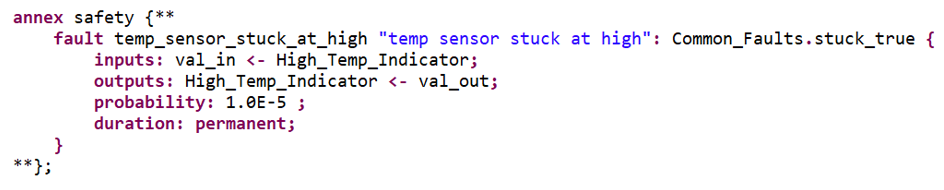
\includegraphics[width=0.9\textwidth]{images/tempSensorFault.PNG}
	\end{center}
	\vspace{-2em}
	\caption{Fault on Temperature Sensor Defined in the Safety Annex for AADL}
	\label{fig:tempSensorFault}
	\vspace{-2em}
\end{figure*}

The Safety Annex provides a way to weave the faults into the nominal model by use of the \emph{inputs} and \emph{outputs} keywords. This allows users to define a fault and attach it to the output of a component. The fault shown in Figure~\ref{fig:tempSensorFault} is defined to be a {\em permanent} fault and has probability of occurrence set at $1.0 \times 10^{-5}$. If the fault is active, the error can possibly violate the guarantees of this component or the assumptions of downstream components~\cite{stewart2020safety}. The activation of a fault is not up to the user, but instead left up to the model checker, JKind, to determine if the activation of this fault will contribute to a violation of higher level guarantees. If so, it can be activated during the analysis.





\begin{center}
\resizebox{0.5\textwidth}{!}{%
    \begin{tabular}{ | c | c | c |}
      \hline
      \thead{Component} & \thead{Layer of Analysis} & \thead{Guarantee}\\
      \hline
      ReactorSys & Top &  \makecell{Safety Property $P$: \\ $((temp$ $>$ $T_t)$ $\lor$ $ (pressure$ $>$ $ T_p)$  $\lor$ $ (radiation$ $>$ $ T_r))$ \\ $\iff SHUTDOWN$}    \\
      \hline
      TempSys & Leaf  &  \makecell{Guarantee $G_t$: \\  $temp$ $>$ $ T_t \iff SHUTDOWN$}   \\
      \hline
      PressureSys & Leaf  &  \makecell{Guarantee $G_p$: \\ $pressure$ $>$ $ T_p \iff SHUTDOWN$}    \\
	\hline
      RadiationSys & Leaf  &  \makecell{Guarantee $G_r$: \\ $radiation$ $>$ $ T_r \iff SHUTDOWN$}   \\
      \hline
    \end{tabular}}
  \end{center}

\begin{center}
\resizebox{0.5\textwidth}{!}{%
    \begin{tabular}{ | c | c | c |}
      \hline
      \thead{Component} & \thead{Layer of Architecture} & \thead{Faults}\\
      \hline
      Temp Sensors (3) & \makecell{Leaf \\ Components} & \makecell{$f_{t}$: fail low}  \\
      \hline
	Pressure Sensors (3) & \makecell{Leaf \\ Components} & \makecell{$f_{p}$: fail low}  \\
      \hline
	Radiation Sensors (3) & \makecell{Leaf \\ Components} & \makecell{$f_{r}$: fail low}  \\
      \hline
    \end{tabular}}
  \end{center}



\subsection{Using this Example in the Generation of Minimal Cut Sets}
Step by step, we outline how minimal cut sets are generated through the \aivcalg algorithm using the sensor system as an example. For ease of reference, a table is provided giving model elements of interest in the sensor example. We refer to these throughout this section. Note: the thresholds vary for pressure, temperature, and radiation. These are given as constants $T_p$, $T_t$, and $T_r$ respectively. We also do not list all guarantees and assumptions that are in the model, but only the ones of interest for this analysis.

\begin{center}
\resizebox{\textwidth}{!}{%
    \begin{tabular}{ | c | c | c |}
      \hline
      \thead{Component} & \thead{Layer of Analysis} & \thead{Guarantee}\\
      \hline
      ReactorSys & Top &  \makecell{Safety Property $P$: \\ $((temp$ $>$ $T_t)$ $\lor$ $ (pressure$ $>$ $ T_p)$  $\lor$ $ (radiation$ $>$ $ T_r))$ \\ $\iff SHUTDOWN$}    \\
      \hline
      TempSys & Leaf  &  \makecell{Guarantee $g_t$: \\  $temp$ $>$ $ T_t \iff SHUTDOWN$}   \\
      \hline
      PressureSys & Leaf  &  \makecell{Guarantee $g_p$: \\ $pressure$ $>$ $ T_p \iff SHUTDOWN$}    \\
	\hline
      RadiationSys & Leaf  &  \makecell{Guarantee $g_r$: \\ $radiation$ $>$ $ T_r \iff SHUTDOWN$}   \\
      \hline
    \end{tabular}}
  \end{center}

\begin{center}
%\resizebox{\textwidth}{!}{%
    \begin{tabular}{ | c | c | c |}
      \hline
      \thead{Component} & \thead{Layer of Architecture} & \thead{Faults}\\
      \hline
      Temp Sensors (3) & \makecell{Leaf \\ Components} & \makecell{$f_{t}$: fail low}  \\
      \hline
	Pressure Sensors (3) & \makecell{Leaf \\ Components} & \makecell{$f_{p}$: fail low}  \\
      \hline
	Radiation Sensors (3) & \makecell{Leaf \\ Components} & \makecell{$f_{r}$: fail low}  \\
      \hline
    \end{tabular}
  \end{center}

The first two steps of this process are performed top down in conjunction with JKind analysis over a program. Thus, the top layer is analyzed first, then the next and so on. Steps 3 and 4 proceed after all MIVCs for each layer have been generated. We walk through this sensor system example in this fashion. 

\textbf{Step 1a: Preprocessing top layer.} The preprocessing step inserts specific MIVC elements into the Lustre program. The MIVC elements are the model elements considered in the constraint system for a given property. The Safety Annex provides the means to define a fault over the output of a component. This fault is given an unassigned \emph{trigger} Boolean literal in Lustre. If the trigger literal is true, the output of the component is changed. If not, the output remains equivalent to the nominal output of this component~\cite{stewart2020safety, Stewart17:IMBSA}. This trigger in Lustre is called a \emph{fault activation literal}. The IVC elements required in order to perform this transformation are these fault activation literals as well as guarantees. The basic rules used to insert these additional literals into Lustre depend on the analysis layer of that is being formed in Lustre and are as follows. 
\begin{itemize}
\item Leaf layer of analysis: only fault activation literals are added.
\item Middle or top layers: guarantees are added and if a direct subcomponent is a leaf component of the architecture and faults are defined on its outputs, then these faults are also added.
\end{itemize}

At the top level, guarantees of the sensor subsystems are the IVC elements.
$$\boxed{g_t, g_p, g_r}$$

There are distinct constraint systems, one for each property being proved. In this system at the top layer, there is a single property $P$; this results in the following constraint system. 
$$\boxed{C = \{g_t, g_p, g_r, \neg P\}}$$

\textbf{Step 2a: Generate all MIVCs for the constraint system at the top layer.} In order to prove $P$, all three guarantees from the sensor subsystem level are required. 
$$\boxed{MIVC(P) = \{g_t, g_p, g_r\}}$$. 

\textbf{Step 1b: Preprocessing leaf layer.} Model elements for the IVC algorithm consideration are the faults for each sensor, for instance temperature sensors:
$$\boxed{f_{t1}, f_{t2}, f_{t3}}$$ 

The resulting constraint system for the temperature sensor subsystem layer is:
$$\boxed{C = \{\neg f_{t1}, \neg f_{t2}, \neg f_{t3}, \neg g_t\}}$$

\textbf{Step 2b: Generate all MIVCs for the constraint system at the leaf layer.} Due to the majority voting mechanism, the MIVCs show all possible pairs of faults restricted to \emph{false}. This means, if any combination of two faults do not occur, then the guarantees at the temperature sensor subsystem level are satisfied. 
$$\boxed{
	\begin{aligned}
		MIVC_1(g_t) = \{\neg f_{t1}, \neg f_{t2}\} \\
		MIVC_2(g_t) = \{\neg f_{t1}, \neg f_{t3}\} \\
		MIVC_3(g_t) = \{\neg f_{t2}, \neg f_{t3}\}
	\end{aligned}
}$$

At this point, all MIVCs have been successfully generated (which is a requirement of the following algorithms) and we can move on to the generation of minimal cut sets. 

\textbf{Step 3a: Generate MCSs using a hitting set algorithm at the top layer.} Our single MIVC in this case will reveal three associated MCSs. (Notice: $MCS_1 \cap MIVC(P) \neq \emptyset$, and same for $MCS_2$ and $MCS_3$, thus these are hitting sets.)
 $$\boxed{
	\begin{aligned}
		MCS_1(top) = \{g_t\} \\
		MCS_2(top) = \{g_p\} \\
		MCS_3(top) = \{g_r\}
	\end{aligned}
}$$

\textbf{Step 4a: Transform MCSs into MinCutSets at the top layer.} Given that only guarantees are found in the MCSs at this layer, recursion is used to find the faults that cause violation of these guarantees. Using this recursion on $MCS_1$, we show the process further. 

\textbf{Step 3b: Generate MCSs using a hitting set algorithm at the leaf layer.} In step 2b, we found all MIVCs for the contract $g_t$ and send these to the hitting set algorithm. The resulting MCSs are: 
 $$\boxed{
	\begin{aligned}
		MCS_1(leaf) = \{\neg f_{t1}, \neg f_{t2}\} \\
		MCS_2(leaf) = \{\neg f_{t1}, \neg f_{t3}\} \\
		MCS_3(leaf) = \{\neg f_{t2}, \neg f_{t3}\}
	\end{aligned}
}$$

Only constrained faults are found in these MCSs, so we simply remove those constraints and have found the MinCutSets for the contracts $g_t$. These are returned and replace this contract in the top layer $MCS_1(top)$. Here is the end result for $MCS_1(top)$; this can be understood as three of the total minimal cut sets for $P$. 

\begin{equation*}
MCS_1(top) \rightarrow \left\{ \,
\begin{IEEEeqnarraybox}[][c]{l?s}
\IEEEstrut
MinCutSet_1(P) = \{f_{t1}, f_{t2}\}, \\
MinCutSet_2(P) = \{f_{t1},  f_{t3}\}, \\
MinCutSet_3(P) = \{f_{t2}, f_{t3}\}
\IEEEstrut
\end{IEEEeqnarraybox}
\right.
\end{equation*}

After all replacements have been made, we are left with all minimal cut sets for the property of interest ($P$ in this example). 

\end{comment}










\section{Formalization}
\label{sec:formalization}
Given a state space $U$, a transition system $(I,T)$ consists of an
initial state predicate $I : U \to \bool$ and a transition step
predicate $T : U \times U \to \bool$.
We define the notion of
reachability for $(I, T)$ as the smallest predicate $\reach : U \to
\bool$ which satisfies the following formulas:
\begin{gather*}
  \forall u.~ I(u) \Rightarrow \reach(u) \\
  \forall u, u'.~ \reach(u) \land T(u, u') \Rightarrow \reach(u')
\end{gather*}
A safety property $P : U \to \bool$ is a state predicate. A safety
property $P$ holds on a transition system $(I, T)$ if it holds on all
reachable states, i.e., $\forall u.~ \reach(u) \Rightarrow P(u)$,
written as $\reach \Rightarrow P$ for short. When this is the case, we
write $(I, T)\vdash P$. We assume the transition relation has the structure of a top level conjunction. Given $T(u, u') = T_1(u,u') \land \cdots T_n(u,u')$ we will write $T = \land_{i=1..n}$ for short. By further abuse of notation, $T$ is identified with the set of its top-level conjuncts. Thus, $T_i \in T$ means that $T_i$ is a top-level conjunct of $T$, and $S\subseteq T$ means all top level conjuncts of $S$ are top-level conjuncts of $T$. When a top-level conjunct $T_i$ is removed from $T$, we write $T \setminus \{T_i\}$

The set of all nominal guarantees of the system $G$ consists of conjunctive constraints $g \in G$. Given no faults (i.e., nominal system) and a transition relation $T$ consisting of conjunctive constraints $T_i$ as defined in section~\ref{sec:prelim}, each $g$ is one of the transition constraints $T_i$ where:

\begin{gather}
T = g_1 \land  g_2 \land \cdots \land g_n
\label{eq:Tn}
\end{gather}

We consider an arbitrary layer of analysis of the architecture and assume the property holds of the nominal relation $(I,T) \vdash P$. Given that our focus is on safety analysis in the presence of faults, let the set of all faults in the system be  denoted as $F$. A fault $f \in F$ is a deviation from the normal constraint imposed by a guarantee. Without loss of generality, we associate a single fault and an associated fault probability with a guarantee. Each fault $f_i$ is associated with an \emph{activation literal}, $\mathit{af}_i$, that determines whether the fault is active or inactive. %Any ``faults" in a mid-layer are simply violated guarantees, or deviations from normal behavior. 

%The faults in the safety annex are defined on leaf level components. Thus, for the lowest analysis layer, we must take into consideration faults and the guarantees their activation may violate. A fault $f \in F$ is a deviation from the normal constraint imposed by a guarantee. For the purposes of this paper, each guarantee at the leaf layer of analysis has an associated fault. 

To consider the system in the presence of faults, consider a set $GF$ of modified guarantees in the presence of faults and let a mapping be defined from activation literals $\mathit{af}_i \in AF$ to these modified guarantees $\mathit{gf}_i \in GF$. 
\begin{center}
$\mathit{gf}_i =$ \textit{if} $\mathit{af}_i$ \textit{then} $f_i$ \textit{else} $g_i$\\
\label{eq:sigma}
\end{center}

The transition system is composed of the set of modified guarantees $GF$ and a set of conjunctions assigning each of the activation literals $\mathit{af}_i \in AF$ to false: 

\begin{gather}
T' = \mathit{gf}_1 \land \mathit{gf}_2 \land \cdots \land \mathit{gf}_n \land \neg \mathit{af}_1 \land \neg \mathit{af}_2 \land \cdots \land \neg \mathit{af}_n
\label{eq:T}
\end{gather}

\begin{theorem} If $(I,T) \vdash P$ for $T$ defined in equation~\ref{eq:Tn}, then $(I,T') \vdash P$ for $T'$ defined in equation~\ref{eq:T}.
\begin{proof}
By the mapping of each constrained activation literal $\neg \mathit{af}_i$ to the associated guarantee $g_i$ and the weakening of the antecedent by introduction of the activation literals, the result is immediate.
\end{proof}
\end{theorem}

Consider the elements of $T$ as a set $GF \cup AF$, where $GF$ are the potentially faulty guarantees and $AF$ consists of the activation literals that determine whether a guarantee is faulty. This is a set that is considered by an SMT solver for satisfiability during the model checking engine procedures. 

Given the extended transition system $T'$, if the $\mathit{af}_i \in \mathit{AF}$ are unconstrained and this causes violation of $P$, a counterexample is returned. For each counterexample, we can partition $\mathit{AF}$ into two sets which we call {\em non-faulty variables (NFV)} and {\em faulty variables (FV)}.  The set $\mathit{NFV}$ consists of a set of variables that are constrained to be false throughout the counterexample, and $\mathit{FV}$ contains those that can be non-deterministically assigned at some point in the trace. By mapping some of the variables in $\mathit{AF}$ to false, we know that associated guarantees in $\mathit{GF}$ are non-faulty for all considered executions. We define $T'(\mathit{NFV})$ as a relaxation of $T'$:

\begin{gather*}
T'(\mathit{NFV}) = \mathit{gf}_1 \land \mathit{gf}_2 \land \cdots \land \mathit{gf}_n \land \bigwedge \{\neg \mathit{af}_i | \mathit{af}_i \in \mathit{NFV} \}
\end{gather*}

The activation literals constrained to be false in $\mathit{NFV}$ cause their associated guarantees to be valid. When $\mathit{af}_i \in \mathit{AF}$ are given a true valuation (and thus are in $\mathit{NF}$), the associated guarantee will be violated. This violation causes the output that the guarantee constrains to become non-deterministic. The Boolean variables in $\mathit{FV}$ correspond to Boolean variables in the fault tree. 

%Given the extended transition system in Equation~\ref{eq:T}, if the $\mathit{af}_i \in \mathit{AF}$ are unconstrained and this causes violation of $P$, a counterexample is returned.  This counterexample is a partition of guarantees $\mathit{GF}$ into disjoint sets:  $\mathit{GF} = \mathit{NFV} \cup \mathit{FV}$. The set $\mathit{NFV}$ consists of nonfaulty variables: the associated $\mathit{af}_i$ are mapped to {\em false} in the counterexample, and the set $\mathit{FV}$ consists of faulty variables: the associated $\mathit{af}_i$ are mapped to {\em true} in the counterexample. In the remainder of this section, we assume that all $\mathit{af}_i \in \mathit{AF}$ are nondeterministically unconstrained and when active, cause the associated guarantee to be violated. Thus the output that the guarantee constrains becomes nondeterministic when the associated $\mathit{af}_i$ is true.


%%						DEFINE FT/FF
\begin{definition}
A fault tree $\mathit{FT}$ is a pair $(r, \mathcal{L})$ where:
\begin{itemize}
\item[] $r$: the root is a guarantee $r \in P$ corresponding to a violated property
\item[] $\mathcal{L}$: a Boolean equation containing faulty vars $\mathcal{L} \subseteq \mathit{FV}$
\end{itemize}
%The fault tree $\mathit{FT}$ is a Boolean equation in disjunctive normal form (DNF): $(r, \mathcal{L}) = r \lor \mathcal{L} = r \lor C_1 \lor \cdots \lor C_n$ for conjunctions $C_i$. 
\end{definition}

The terms $\mathit{af}$  in the Boolean formula $\mathcal{L}$ may be extracted as the set of leaf nodes of the fault tree. 

\begin{definition} 
A fault tree $FT = (r, \mathcal{L})$ is valid if and only if $(r, \mathcal{L})$ is satisfiable with a true valuation for $r$ and for all $\mathit{af} \in \mathcal{L}$. 
\label{def:validFT}
\end{definition}


Each layer of the architecture may contain multiple properties $P$. The subset $\pi$ of $P$ are the properties which have an associated fault tree and are either top level safety properties themselves or are used to prove the properties of a parent level. Due to this multiplicity, we do not compose single fault trees per layer, but rather forests of trees.

\begin{definition}
A fault forest $\mathit{FF}$ is a set of fault trees.
\end{definition}

\begin{definition}
A fault forest $\mathit{FF}$ is valid if and only if for all $\mathit{FT} \in \mathit{FF}$, $\mathit{FT}$ is valid.
\label{def:validFF}
\end{definition}


% 					COMPOSE FAULT FORESTS:
%%%%%%%%%%%%%%%%
%Let $n$ be the number of properties for some parent component $p$ and let $m$ be the number of properties for some child component $c$. Then the fault forest $\mathit{FF}_c$ is a mapping $\mathit{FF}_c : S_1 \rightarrow B$ for $S_1 = \{1,2,\dots,m\}$ and the set of Boolean equations $B$ and $\mathit{FF}_p: S_2 \rightarrow B$ for $S_2 = \{1,2,\dots n\}$. We use the notation $\mathit{seq(B)}$ to describe a sequence of Boolean equations.
%%%%%%%%%%%%%%%%%%%%%

%							SET UP FOR COMPONENT DEFINITION
A counterexample is a trace. That trace is a valuation that splits $\mathit{AF}$ into disjoint sets $\mathit{NFV} \cup \mathit{FV}$. Each counterexample determines a set $\mathit{FV}$ with respect to a property $\pi_i \in \pi$. This defines an associated fault tree $\mathit{FT}_i \in \mathit{FF}$ where the root of the tree is the property $\pi_i$.  

On the other hand, we also want to describe the non-faulty variables that are required for the proof of all $\pi_i \in \pi$ in order to have a valid component throughout composition. These are used in the relaxation of $T'$ and can be stated as $(I, T'(\mathit{NFV})) \vdash \pi$. A valid component has the potential to either prove pertinent properties (non-faulty variables) or violate properties (faulty variables), depending on the valuation of activation literals. 

%%					DEFINE COMPONENT
\begin{definition}
A component is the tuple $\mathit{Comp}(M, \mathit{FF}, \mathit{NFV}, \pi)$ where:
\begin{itemize}[label=\textbullet]
\item $M$: the model consisting of the set of child properties $P_c$ extended with non-deterministic faults: $\mathit{gf}_i \in P_c$ where $\mathit{gf}_i =$ \textit{if} $\mathit{af}_i$ \textit{then} $\mathit{f}_i$ \textit{else} $g_i$
\item $\mathit{FF}$: the ordered set of fault trees for this component
\item $\mathit{NFV}$: the set of non-faulty variables 
\item properties $\pi \subseteq P$ such that $(I, T'(\mathit{NFV})) \vdash \pi$
\end{itemize}
and $\mathit{FT}_i \in \mathit{FF}$ corresponds to $\pi_i \in \pi$ for each of the $i$ properties.  
\end{definition}


%%					EXAMPLE OF COMPONENT DEF AND FF/FT DEFS
As an example, we return to the sensor system described in Section~\ref{sec:example}. The component {\em Pressure Subsystem} can be defined as follows. 

\begin{itemize}[label=\textbullet]
\item $M = \{\mathit{gf}_{p1}, \mathit{gf}_{p2}, \mathit{gf}_{p3}\}$. These are the child properties of the pressure subsystem extended with faults. 
\item $\mathit{FT} = (r, \mathcal{L}) = (\neg G_p, (\mathit{af}_{p1} \land \mathit{af}_{p2}) \lor (\mathit{af}_{p1} \land \mathit{af}_{p3}) \lor (\mathit{af}_{p2} \land \mathit{af}_{p3}) $: the fault tree leaf formula has all pairwise combinations of active sensor faults. The fault forest for this component consists only of this single tree.
\item $\mathit{NFV} = \{\mathit{gf}_{p1}, \mathit{gf}_{p2}, \mathit{gf}_{p3}\}$: in this example, all three guarantees must be non-faulty in order to prove the property $\pi$.
\item $\pi = \{G_p\}$: the only property of this subsystem is required for the proof of the top level safety property. Notice that $(I, T'(\mathit{NFV})) \vdash \pi$.
\end{itemize}


%%				DEFINE COMPOSITION OF COMPONENTS
\begin{definition}
The composition of child component $\mathit{Comp}_c$ and parent component $\mathit{Comp}_p$:
$Comp_c(M_c, \mathit{FF}_c, \mathit{NFV}_c, \pi_c) \circ Comp_p(M_p, \mathit{FT}_p, \mathit{NFV}_p, \pi_p) = Comp_\circ(M', \mathit{FF}', \mathit{NFV}', \pi')$ where:
\begin{itemize}[label=\textbullet]
\item $M' = M_c \cup M_p$ is the iterative enlargement of the model,
\item $\mathit{FF}_c \circ \mathit{FF}_p$ is the composed fault forest
\item $\mathit{NFV}' = \mathit{NFV}_c \cup \mathit{NFV}_p$ is the set of non-faulty variables
\item $\pi' = \pi_c \cup \pi_p$ are valid properties such that $(I, T'(\mathit{NFV}')) \vdash \pi'$.
\end{itemize}
\end{definition}


%%				NFV |- PI
Given that in child and parent components, the properties $\pi$ can be derived from the non-faulty variables, we show that this relationship holds after composition. To state $(I, T'\mathit{NFV})) \vdash \pi$, we use the shorthand $\mathit{NFV} \vdash \pi$. 

\begin{theorem} If $\mathit{NFV}_c \vdash \pi_c$ and $\mathit{NFV}_p \vdash \pi_p$, then $\mathit{NFV}' \vdash \pi'$
\begin{proof}
Assume antecedent. Let $p' \in \pi'$. If $p' \in \pi_c$ then $\mathit{NFV}_c \vdash p'$ and likewise if $p' \in \mathit{NFV}_p$, then $\mathit{NFV}_p \vdash p'$. In either case, $\mathit{NFV}_c \cup \mathit{NFV}_p = \mathit{NFV}' \vdash \pi'$.
\end{proof}
\end{theorem} 

%%								DEFINE PHI for trees
To show that the composition of fault trees results in a valid fault tree, we define a mapping. Let $\phi$ be a function $\phi : B \times B \rightarrow B$ for Boolean equations $B$. We use this mapping to define the composition of parent and child component fault trees: $\mathit{FT}_c = (r_c, \mathcal{L}_c)$ and $\mathit{FT}_p = (r_p, \mathcal{L}_p)$.

\begin{gather}
\mathit{FT}_c \circ \mathit{FT}_p = \phi(\mathit{FT}_c, \mathit{FT}_p) =\begin{cases} 
      (r_p, \mathcal{L}_p(r_c, \mathcal{L}_c)) & r_c \in \mathcal{L}_p \\
      (r_p, \mathcal{L}_p) & r_c \not\in \mathcal{L}_p \\
   \end{cases}
\label{eq:phi}
\end{gather}

where $\mathcal{L}_p(r_c, \mathcal{L}_c)$ is the replacement of $r_c$ in $\mathcal{L}_p$ with $\mathcal{L}_c$.

%%%%5										COMPOSITION OF FT IS VALID
We work under the {\em monotonicity assumption}, commonly adopted in safety analysis, that an additional fault can not prevent the violation of the property. 

\begin{lemma} If $\mathit{FT}_c$ and $\mathit{FT}_p$ are valid fault trees, then their composition $\phi(\mathit{FT}_c, \mathit{FT}_p)$ is also a valid fault tree. 
\begin{proof}
Assume $\mathit{FT}_c$ and $\mathit{FT}_p$ are valid fault trees and let $\phi$ be defined as in (\ref{eq:phi}).  

 $\forall \mathit{af} \in \mathit{FT}_c$, $\mathit{af}$ has a true valuation and is added to the formula $\mathit{FT}_p$. By the monotonicity assumption and Definition~\ref{def:validFT}, the resulting formula is satisfiable. 
\end{proof}
\label{lemma:validTree}
\end{lemma}

%%%%%									DEFINE PHI FOR FORESTS
Since each layer of the model may contain multiple properties, we wish to extend these formalisms to forests. We begin by extending the definition of the composing function $\phi$. Let $n$ be the number of properties for some parent component $p$ and let $m$ be the number of properties for some child component $c$. Then the parent fault forest $\mathit{FF}_p$ is a mapping $\mathit{FF}_p : S_1 \rightarrow B$ for $S_1 = \{1,2,\dots,m\}$ and the set of Boolean equations $B$ and $\mathit{FF}_c: S_2 \rightarrow B$ for $S_2 = \{1,2,\dots n\}$. 

Let $\phi_F$ be a function $\phi _F: \mathit{seq(B)} \times \mathit{seq(B)} \rightarrow \mathit{seq(B)}$ for sequences of Boolean equations $\mathit{seq(B)}$. We use this function to define the composition of parent and child component fault forests $\mathit{FF}_p = \{(r_{p1},\mathcal{L}_{p1}), \dots, (r_ {pm}, \mathcal{L}_{pm})\}$ and $\mathit{FF}_c = \{(r_{c1},\mathcal{L}_{c1}), \dots, (r_ {cn}, \mathcal{L}_{cn})\}$. $\phi_F$ is a mapping such that for all $i \in S_1$ and for all $j \in S_2$: 

\begin{gather}
\mathit{FF}_c \circ \mathit{FF}_p = \phi_F(\mathit{FF}_c, \mathit{FF}_p) =\begin{cases} 
      (r_{pi}, \mathcal{L}_{pi}(r_{cj}, \mathcal{L}_{cj})) & r_{cj} \in \mathcal{L}_{pi} \\
      (r_{pi}, \mathcal{L}_{pi}) & r_{cj} \not\in \mathcal{L}_{pi} \\
   \end{cases}
\end{gather}

where $\mathcal{L}_p(r_c, \mathcal{L}_c)$ is the replacement of $r_c$ in $\mathcal{L}_p$ with $\mathcal{L}_c$.

Each literal in the formula $\mathcal{L}_p$ is a fault activation literal $\mathit{af}_i$. If $\mathit{af}_i$ has an associated guarantee $\mathit{gf}_i$ in the set of child roots $r_c$, then the mapping $\phi_F$ will replace $\mathit{af}_i$ in $\mathcal{L}_p$ with the leaf formula of the child root $\mathit{gf}_i$.  The resulting fault forest is a sequence of fault trees $\mathit{FF} = \{(r_{pk}, \mathcal{L}_{k}): k = 1,\dots,m\}$. The roots of the resulting forest are the same roots as  the parent forest while the leaf formulae may change based on replacement. 


%%							EXAMPLE PHI MAPPING WITH PARENT AND CHILD

\begin{figure}[h!]
	\begin{center}
		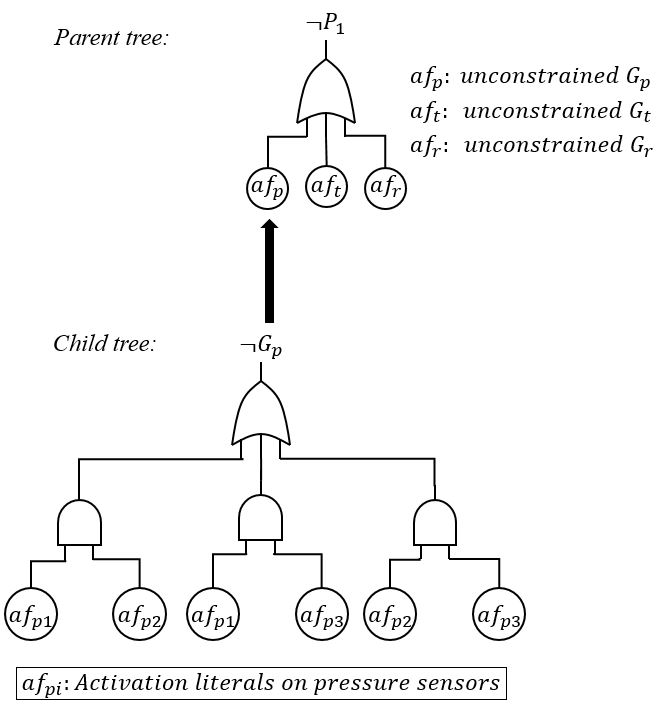
\includegraphics[width=0.5\textwidth]{images/faultCompEx.JPG}
	\end{center}
	\caption{Sensor System Composition of Fault Trees}
	\label{fig:sensorSysComp}
\end{figure}
We return to the sensor system example to illustrate this mapping. Graphically, this is represented in Figure~\ref{fig:sensorSysComp}.  The top level (parent) component is defined as: $\mathit{Comp}_p (M_p, \mathit{FF}_p, \mathit{NFV}_p, \pi_p)$ and $\mathit{FF}_p = \{(\neg P, \mathit{af}_p \lor \mathit{af}_t \lor \mathit{af}_r)\}$ where each activation literal is associated with the unconstrained guarantees $G_p$, $G_t$, and $G_r$. The child layer has a fault forest consisting of three fault trees, one for each subsystem. 

The pressure subsystem fault tree is $\mathit{FT}_{p} = (\neg G_p, (\mathit{af}_{p1} \land \mathit{af}_{p2}) \lor (\mathit{af}_{p1} \land \mathit{af}_{p3}) \lor (\mathit{af}_{p2} \land \mathit{af}_{p3}) $. The leaf formulae for each subsystem tree corresponds to pairwise combinations of active sensor faults. We now show the composition of the pressure subsystem child and top level parent fault trees. 

The mapping $\phi_F$ iterates through each tree in the parent forest -- in this case, we have only one. Then for each parent tree it iterates through the Boolean formulae in $\mathcal{L}$. If there is a match between a child root and a parent leaf, the replacement is made.
Thus, $\mathit{af}_p$ will be replaced with $(\mathit{af}_{p1} \land \mathit{af}_{p2}) \lor (\mathit{af}_{p1} \land \mathit{af}_{p3}) \lor (\mathit{af}_{p2} \land \mathit{af}_{p3})$. This replacement is done for each leaf formula in $\mathcal{L}_p$ from the parent fault forest. 

We represent the unconstrained (violated) guarantee as $\neg G_p$ and it is associated with the fault activation literal $\mathit{af}_p$. The end result of the replacement is easy to see.

%%%%5										COMPOSITION OF FF IS VALID
\begin{lemma} If $\mathit{FF}_c$ and $\mathit{FF}_p$ are valid fault forests, then their composition $\phi(\mathit{FF}_c, \mathit{FF}_p)$ is also a valid fault forest. 
\begin{proof}
By iterative application of Lemma~\ref{lemma:validTree}, the result is immediate.
\end{proof}
\label{lemma:validForest}
\end{lemma}

Thus far, we have proven that a single layer of composition produces valid fault trees (or forests), but to perform this analysis across $n$ layers of architecture we show inductively that the resulting fault forest is valid. 

The notation $\phi_F^n$ indicates the iterated function $\phi_F$ which is a successive application of $\phi_F$ with itself $n$ times. Assume the fault forest $\mathit{FF}_0$ is obtained at the leaf level of the architecture.

\begin{theorem} If $\phi_F^n(\mathit{FF}_{n-1}, \mathit{FF}_n)$ is a valid fault forest, then $\phi^{n+1}(\mathit{FF}_{n}, \mathit{FF}_{n+1})$ is a valid fault forest.
\begin{proof}

Base case: Each fault forest per layer is valid by construction. By Lemma~\ref{lemma:validForest}, $\phi_F(\mathit{FF}_{0}, \mathit{FF}_1)$ is a valid fault forest.

Inductive assumption: Assume $\phi_F^n(\mathit{FF}_{n-1}, \mathit{FF}_n)$ is a valid fault forest.
\begin{equation*}
\begin{split}
\phi_F^{n+1}(\mathit{FF}_{n}, \mathit{FF}_{n+1}) &= ((\mathit{FF}_0 \circ \mathit{FF}_1) \circ \mathit{FF}_2) \circ \cdots \circ \mathit{FF}_n) \circ \mathit{FF}_{n+1})) \\
  &= \phi_F^n(\mathit{FF}_{n-1}, \mathit{FF}_n) \circ \mathit{FF}_{n+1}
\end{split}
\end{equation*}

%$\phi_F^{n+1}(\mathit{FF}_{n}, \mathit{FF}_{n+1}) = ((\mathit{FF}_0 \circ \mathit{FF}_1) \circ \mathit{FF}_2) \circ \cdots \circ \mathit{FF}_n) \circ \mathit{FF}_{n+1})) = \phi_F^n(\mathit{FF}_{n-1}, \mathit{FF}_n) \circ \mathit{FF}_{n+1}$. 

By inductive assumption and Lemma~\ref{lemma:validForest}, $\phi_F^{n+1}(\mathit{FF}_{n}, \mathit{FF}_{n+1})$ is a valid fault forest.

\end{proof}
\label{thm:indForest}
\end{theorem}

We know from previous work that composition is conservative. A valid monolithic analysis of the transition system implies that the compositional analysis of that same system is valid, but the converse may not be true~\cite{}. It is likewise the case for composing fault forests. 

Let $S \subseteq \mathit{AF}$ where all $\mathit{af} \in S$ are constrained to true. If $S \cup \{\neg P\}$ is satisfiable, this equates to a valid fault tree. 

\begin{theorem} If $(I,T) \vdash P$ for monolithic verification, then for $S \subseteq \mathit{AF}$, $S \cup \{\neg P\}$ is unsatisfiable.
\begin{proof}
Assume toward contradiction that $(I,T) \vdash P$ and there exists a set $S \subseteq \mathit{AF}$ such that $S \cup \{\neg P\}$ is satisfiable. This implies that there exists a reachable state such that $\neg P$ holds. This contradicts our assumption. 
\end{proof}
\label{thm:sound}
\end{theorem}

As a counterexample to the converse of Theorem~\ref{thm:sound}, consider the following. \danielle{Counterexample here.}

Now that we have the formal foundations laid, we proceed towards the implementation. 






\section{Preliminaries for the Implementation}
\label{sec:prelim}

%%\textbf{Background Information on Toolsuite}
\danielle{My suggestion is to place this at the front of the implementation section. It just seems like it is taking longer to get to the interesting part of the paper by having it here.}

The algorithms in this paper are implemented in the Safety Annex for the Architecture Analysis and Design Language (AADL) and require the Assume-Guarantee Reasoning Environment (AGREE)~\cite{NFM2012:CoGaMiWhLaLu} to annotate the AADL model in order to perform verification using the back-end model checker \jkind~\cite{2017arXiv171201222G}. 

\textbf{Architecture Analysis and Design Language}
We are using the Architectural Analysis and Design Language (AADL) to construct system architecture models of performance-critical, embedded, real-time systems~\cite{AADL_Standard,FeilerModelBasedEngineering2012}. %An AADL model describes a system in terms of a hierarchy of components and their interconnections, where each component can either represent a logical entity (e.g., application software functions, data) or a physical entity (e.g., buses, processors). 
Language annexes to AADL provide a richer set of modeling elements for various system design and analysis needs, and the language definition is sufficiently rigorous to support formal analysis tools that allow for early phase error/fault detection. 

\textbf{Compositional Analysis} 
One way to structure compositional verification is hierarchically: layers of the system architecture are analyzed independently and their composition demonstrates a system property of interest. Compositional verification partitions the formal analysis of a system architecture into verification tasks that correspond into the decomposition of the architecture~\cite{clarke1989compositional}.  A proof consists of demonstrating that the system property is provable given the contracts of its direct subcomponents and the system assumptions~\cite{cofer2012compositional,clarke1989compositional}. When compared to monolithic analysis (i.e., analysis of the flattened model composed of all components), the compositional approach allows the analysis to scale to much larger systems~\cite{NFM2012:CoGaMiWhLaLu,heckel1998compositional,cofer2012compositional}.

\textbf{Assume Guarantee Reasoning Environment}
The Assume Guarantee Reasoning Environment (AGREE) is a tool for formal analysis of behaviors in AADL models and supports compositional verification~\cite{NFM2012:CoGaMiWhLaLu}.  It is implemented as an AADL annex and is used to annotate AADL components with formal behavioral contracts. Each component's contracts includes assumptions and guarantees about the component's inputs and outputs respectively. AGREE translates an AADL model and the behavioral contracts into Lustre~\cite{Halbwachs91:IEEE} and then queries the \jkind model checker to conduct the back-end analysis~\cite{2017arXiv171201222G}. 

\textbf{JKind}
JKind is an open-source industrial infinite-state inductive model checker for safety properties~\cite{2017arXiv171201222G}. Models and properties in JKind are specified in Lustre~\cite{Halbwachs91:IEEE}, a synchronous dataflow language, using the theories of linear real and integer arithmetic. JKind uses SMT-solvers to prove and falsify multiple properties in parallel.

\textbf{Safety Annex for AADL}
The Safety Annex for AADL provides the ability to reason about faults and faulty component behaviors in AADL models~\cite{Stewart17:IMBSA,stewart2020safety}. In the Safety Annex approach, AGREE is used to define the nominal behavior of system components, faults are introduced into the nominal model, and JKind is used to analyze the behavior of the system in the presence of faults. Faults describe deviations from the nominal behavior and are attached to the outputs of components in the system.%The Safety Annex supports behavioral specification of faults and their implicit propagation through behavioral relationships in the model as well as explicit propagation through dependencies. 
To implement the formalism described in Section~\ref{sec:formalization}, we must compute minimal cut sets per layer of analysis, transform them into their related Boolean formula, and compose them. As previously described, Ghassabani et al. developed the \textit{all minimal inductive validity core} algorithm (\aivcalg)~\cite{GhassabaniGW16,Ghassabani2017EfficientGO}. The \aivcalg algorithm gives the minimal set of contracts required for proof of a safety property. If all of these sets are obtained, we have insight into every proof path for the property. Thus, if we violate at least one contract from every MIVC set, we have in essence ``broken" every proof. 
\begin{figure}[h!]
	\begin{center}
		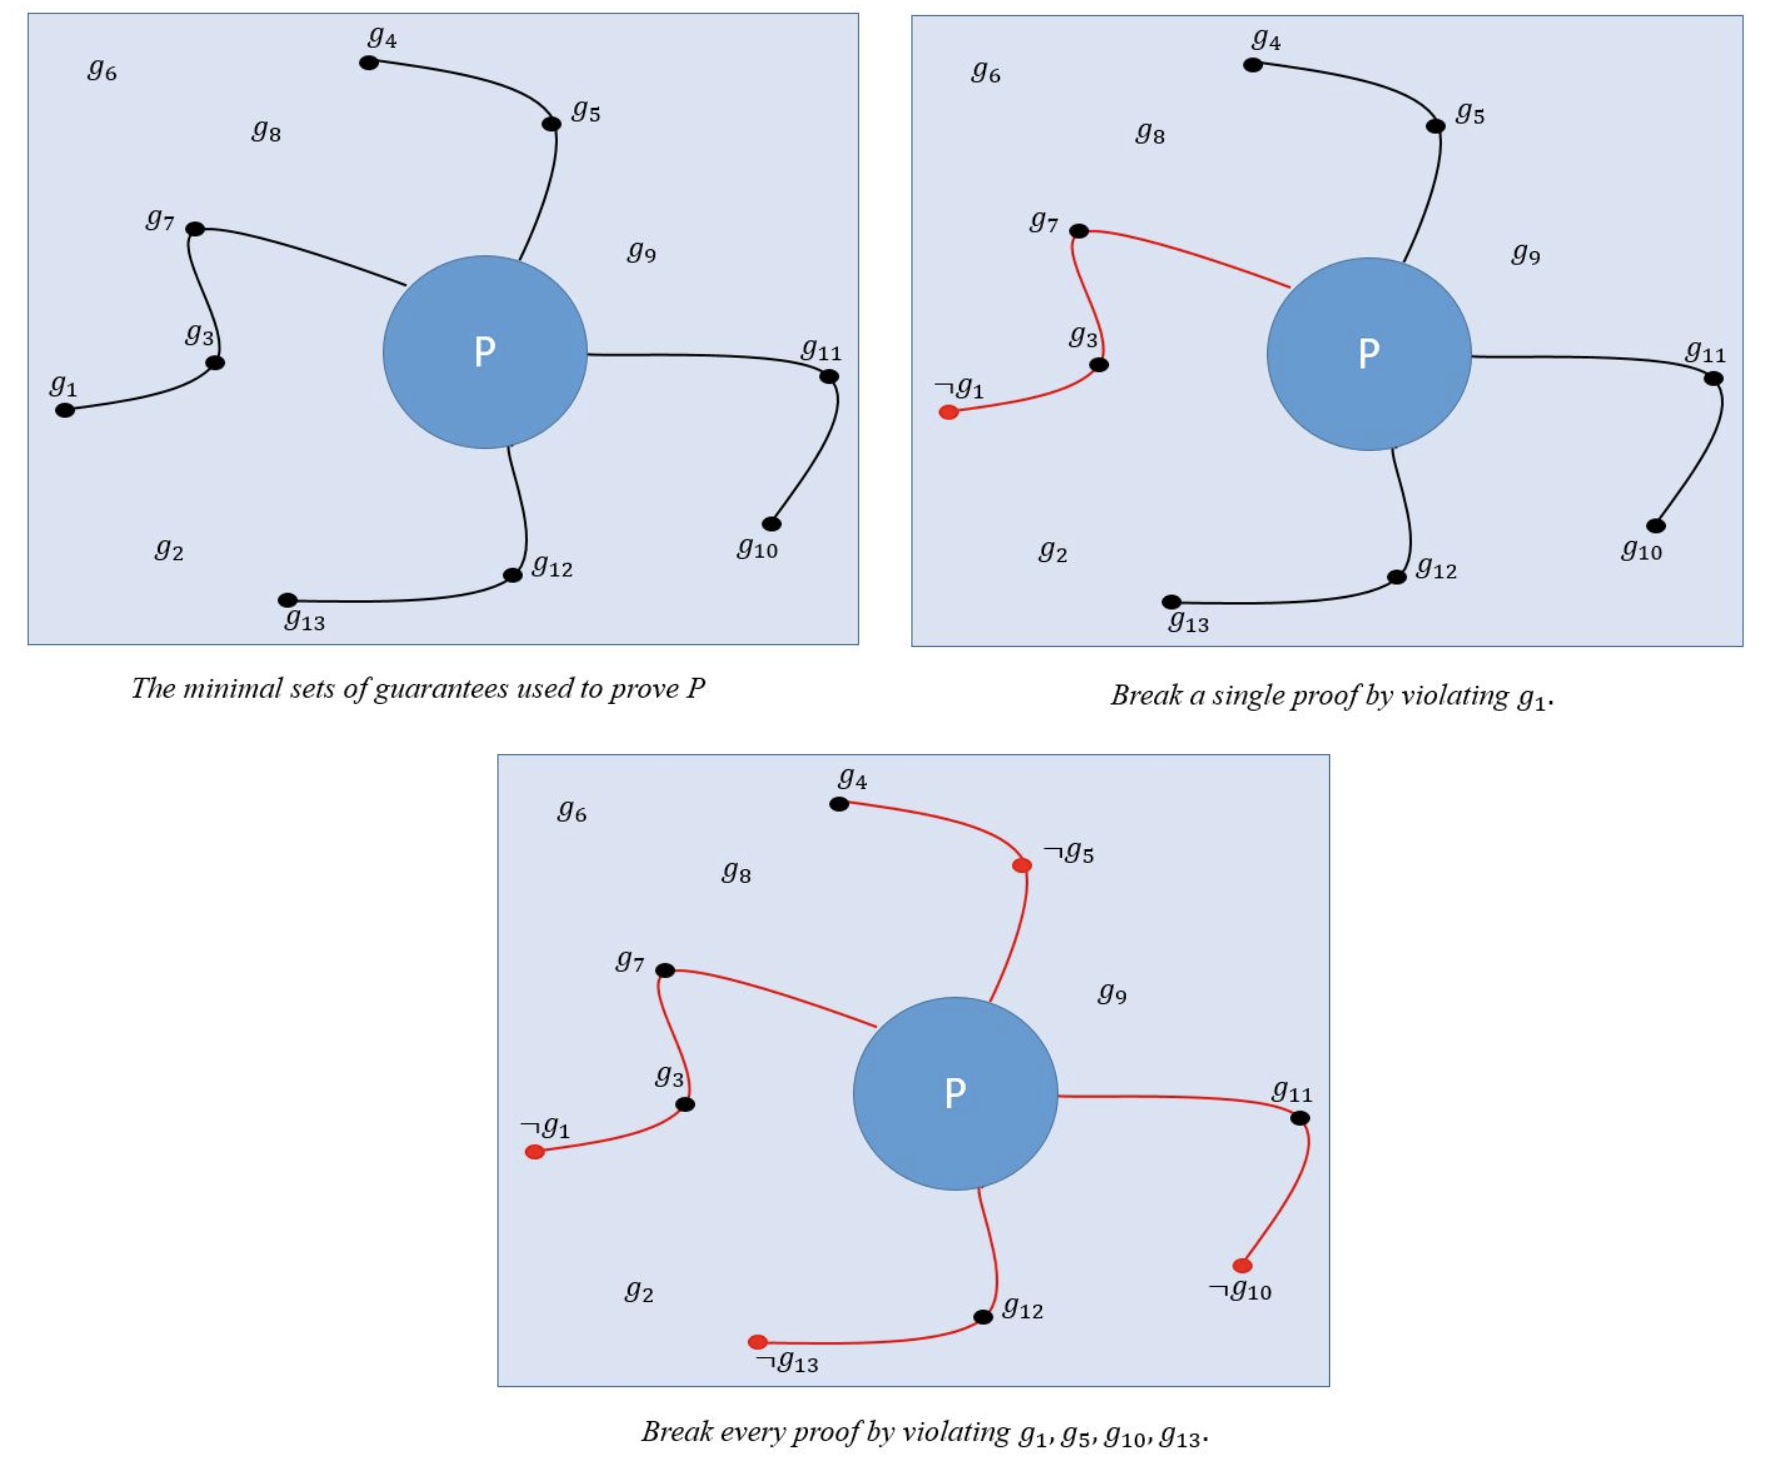
\includegraphics[width=0.9\textwidth]{images/mivcBreaking.png}
	\end{center}
	\caption{Using MIVCs to derive minimal cut sets}
	\label{fig:mivcBreaking}
\end{figure}

In Figure~\ref{fig:mivcBreaking}, we depict this graphically. In the first box (top left), the contracts of the single layer system are $g_1, \dots, g_{13}$. In this example, not all guarantees are needed to prove $P$; one may obtain proof of the property by having only $g_4$ and $g_5$ in the model. The \aivcalg algorithm provides all minimal validity cores which is shown as the lines running through the guarantees. 

One may attempt to violate a proof by violating a guarantee in a single MIVC as shown in the top right of the figure. This does break a proof, but given there are multiple MIVCs, it is not enough. The bottom figure shows our method: violate one guarantee from each MIVC set to ensure that the property can no longer be proven. The key idea is that the hitting sets of all MIVCs produces the minimal cut sets. 

Next we outline the formal background and toolsuite used in the implementation and then describe the algorithm that is implemented in the safety annex for AADL. 

\subsection{Background}
JKind is an open-source industrial infinite-state inductive model checker for safety properties~\cite{2017arXiv171201222G}. Models and properties in JKind are specified in Lustre~\cite{Halbwachs91:IEEE}, a synchronous dataflow language, using the theories of linear real and integer arithmetic. JKind uses SMT-solvers to prove and falsify multiple properties in parallel. The JKind model checker uses {\em
  $k$-induction} which unrolls the property $P$ over $k$ steps of the
transition system.

%\begin{comment}
%For an arbitrary transition system $(I, T)$, computing reachability can be very expensive or even impossible. Thus, we need a more effective way of checking if a safety property $P$ is satisfied by the system. The key idea is to over-approximate reachability. If we can find an over-approximation that implies the property, then the property must hold. Otherwise, the approximation needs to be refined.

A good first approximation for reachability is the property itself.
That is, we can check if the following formulas hold:
\begin{gather}
  \forall s.~ I(s) \Rightarrow P(s)
  \label{eq:1-ind-base} \\
  \forall s, s'.~ P(s) \land T(s, s') \Rightarrow P(s')
  \label{eq:1-ind-step}
\end{gather}
If both formulas hold then $P$ is {\em inductive} and holds over the
system. If (\ref{eq:1-ind-base}) fails to hold, then $P$ is violated
by an initial state of the system. If (\ref{eq:1-ind-step}) fails to
hold, then $P$ is too much of an over-approximation and needs to be
refined.


The JKind model checker uses {\em
  $k$-induction} which unrolls the property $P$ over $k$ steps of the
transition system. For example, 1-induction consists of formulas (\ref{eq:1-ind-base}) and (\ref{eq:1-ind-step}) above, whereas 2-induction consists of the following formulas:
\begin{gather*}
\forall s.~ I(s) \Rightarrow P(s) \\
\forall s, s'.~ I(s) \land T(s, s') \Rightarrow P(s') \\
\forall s, s', s''.~ P(s) \land T(s, s') \land P(s') \land T(s',
  s'') \Rightarrow P(s'')
\end{gather*}
That is, there are two base step checks and one inductive step check.
In general, for an arbitrary $k$, $k$-induction consists of $k$
base step checks and one inductive step check as shown in
Figure~\ref{fig:k-induction} (the universal quantifiers on $s_i$ have
been elided for space). We say that a property is $k$-inductive if it
satisfies the $k$-induction constraints for the given value of $k$.
The hope is that the additional formulas in the antecedent of the
inductive step make it provable.

\begin{figure}
\begin{gather*}
I(s_0) \Rightarrow P(s_0) \\[-2pt]
%
\vdots \\[2pt]
%
I(s_0) \land T(s_0, s_1) \land \cdots \land T(s_{k-2}, s_{k-1})
\Rightarrow P(s_{k-1}) \\[2pt]
%
P(s_0) \land T(s_0, s_1) \land \cdots \land P(s_{k-1}) \land
T(s_{k-1}, s_k) \Rightarrow P(s_k)
\end{gather*}
\caption{$k$-induction formulas: $k$ base cases and one inductive
  step}
\label{fig:k-induction}
\end{figure}

In practice, inductive model checkers often use a combination of the
above techniques. Thus, a typical conclusion is of the form ``$P$ with
lemmas $L_1, \ldots, L_n$ is $k$-inductive''.
%\end{comment}

Each step of induction is sent to an SMT (Satisfiabilty Modulo Theory)-solver to check for \emph{satisfiability}, i.e. there exists a total truth assignment to a given formula that evaluates to true. If there does not exist such an assignment, the formula is considered \emph{unsatisfiable}. %A \emph{constraint system} is a term used to describe the formula with all constraints to the variables. 
A $\mathit{k}$-induction model checker utilizes parallel SMT-solving engines at each induction step to glean information about the proof of a safety property. The transition formula is translated into clauses such that satisfiability is preserved~\cite{een2003temporal}. Expression of the base and induction steps of a temporal induction proof as SAT problems is straightforward and is shown below for step $k$:

\begin{gather*}
I(s_0) \land T(s_0, s_1) \land \cdots \land T(s_{k-1}, s_{k})
\land \neg P(s_{k})
\end{gather*}

When proving correctness it is shown that the formulas are \emph{unsatisfiable}, i.e., the property $P$ is provable. The idea behind finding an {\em inductive validity core} (IVC) for a given property $P$ is based on inductive proof methods used in SMT-based model checking, such as $\mathit{k}$-induction and IC3/PDR~\cite{een2011efficient, kahsai2012incremental}. Generally, an IVC computation technique aims to determine, for any subset $S \subseteq T$, whether $\mathit{P}$ is provable by $\mathit{S}$. A minimal subset that satisfies $\mathit{P}$ is seen as a minimal proof explanation and called a minimal inductive validity core. %Ghassabani et al. demonstrate that the minimization process is as hard as model checking~\cite{Ghassabani2017EfficientGO}, so finding a minimal inductive validity core may not be possible for some model checking problems. 

\begin{definition}
Inductive Validity Core (IVC)~\cite{GhassabaniGW16}: $S \subseteq T$ for $(I, T) \vdash P$ is an Inductive Validity Core, denoted by $\mathit{IVC(P,S)}$, iff $\mathit{(I,S)} \vdash P$.
\end{definition}

\begin{definition}
Minimal Inductive Validity Core (MIVC)~\cite{Ghassabani2017EfficientGO}: $S \subseteq T$ is a minimal Inductive Validity Core, denoted by $\mathit{MIVC(P,S)}$, iff $\mathit{IVC(P,S)} \land \forall T_i \in S$. $(I, S \setminus \{T_i\}) \not \vdash P$.
\end{definition}

The {\em constraint system} consists of the constrained formulas of the transition system and the negation of the property. The \aivcalg algorithm collects all {\em minimal unsatisfiable subsets} (MUSs) of a constraint system generated from a transition system at each induction step~\cite{Ghassabani2017EfficientGO,bendik2018online}. 

\begin{definition}
A Minimal Unsatisfiable Subset (MUS) $M$ of a constraint system $C$ is a set $M \subseteq C$ such that $M$ is unsatisfiable and $\forall c \in M$ : $M \setminus \{c\}$ is satisfiable.
\end{definition}
The MUSs are the minimal explanation of the infeasibility of this constraint system; equivalently, these are the minimal sets of model elements necessary for proof of the safety property.

Returning to our running example, this can be illustrated by the following. Given the constraint system $C = \{G_p, G_t, G_r, \neg P\}$, a minimal explanation of the infeasability of this system is the set $\{G_p, G_t, G_r,\}$. If all three guarantees hold, then $P$ (the disjunction of these guarantees) is provable. 

In the case of an UNSAT system, we may ask: what will correct this unsatisfiability? A related set answers this question: 
\begin{definition}
A Minimal Correction Set (MCS) $M$ of a constraint system $C$ is a subset $M\subseteq C$ such that $C \setminus M$ is satisfiable and $\forall M' \subset M$ : $C \setminus M'$ is unsatisfiable.
\end{definition}
An MCS can be seen to ``correct'' the infeasability of the constraint system by the removal from $C$ the constraints found in an MCS. Returning to the PWR example, the MCSs of the constraint system $C$ are $\mathit{MCS}_1 = \{G_t\}$, $\mathit{MCS}_2 = \{G_p\}$, $\mathit{MCS}_3 = \{G_r\}$. If any single guarantee is violated, a shut down from that subsystem may not get sent when it should and the safety property $P$ will be violated. This corresponds exactly to the definition of a minimal cut set.

For the following definitions, we remind readers of the extended transition system defined in Equation 2 of Section~\ref{sec:formalization} and that the elements of $T'$ are the set $\mathit{GF} \cup \mathit{AF}$ for potentially faulty guarantees $\mathit{GF}$ and activation literals $\mathit{AF}$. We use the notation $\mathit{af} \rightarrow \{\mathit{true}, \mathit{false}\}$ to indicate a constraint on the literal $\mathit{af}$. 

\begin{definition}
A cut set $S$ of a top level event $\neg P$ is a set $S \subseteq \mathit{AF}$ such that $\forall \mathit{af} \in S$, $\mathit{af} \rightarrow \{\mathit{true}\}$ and $S \cup \{\neg P\}$ is satisfiable.
\end{definition}

Intuitively, a cut set is a true valuation for some subset of fault activation literals within a constraint system such that the constraint system is satisfiable given those true valuations.

\begin{definition}
A cut set $S$ is minimal if and only if $\forall \mathit{af} \in S$, $S \setminus \{\mathit{af}\} \cup \{\neg P\}$ is unsatisfiable.
\end{definition}

Our approach in computing minimal cut sets through the use of inductive validity cores is to supply activation literals constrained to be false to the algorithm. The resulting MCSs consist of elements $\neg \mathit{af}_i$. The removal of this constraint from the constraint system results in non-deterministically true activation literals. By the definition of an MCS, we know that $C \setminus \mathit{MCS}$ is satisifiable. This removal of constraints from $C$ removes the {\em false} constraint from each element in the MCS. Liffiton et. al showed that any subset of a satisfiable set is also satisfiable~\cite{liffiton2016fast}, so we know that for set $S$ consisting of elements of MCS with constraints removed, $S \cup \{\neg P\}$ is also satisfiable. This is the definition of a cut set. Minimality comes directly from the definition of a minimal correction set. 

A duality exists between the MUSs of a constraint system and the MCSs as established by Reiter \cite{reiter1987theory}. This duality is defined in terms of \textit{Minimal Hitting Sets} (\textit{MHS}). 
\begin{definition}
A hitting set of a collection of sets $A$ is a set $H$ such that every set in $A$ is ``hit'' by $H$; $H$ contains at least one element from every set in $A$. 
\end{definition}
Every MUS of a constraint system is a minimal hitting set of the system's MCSs, and likewise every MCS is a minimal hitting set of the system's MUSs. This is noted in previous work~\cite{liffiton2016fast, de1987diagnosing} and the proof of such is given by Reiter (Theorem 4.4 and Corollary 4.5)~\cite{reiter1987theory}. For the PWR top level constraint system, it can be seen that each of the MCSs intersected with the MUS is nonempty. This gives the minimal set of guarantees for which, if violated, will cause $P$ to be violated. 

As described in Section~\ref{sec:formalization}, we extend the transition system with fault activation literals. These literals are constrained to {\em false} and the \aivcalg algorithm is invoked. The constraint system for the PWR example is $C = \{\neg\mathit{af}_p, \neg\mathit{af}_t, \neg\mathit{af}_r, \neg P\}$ for activation literal $\mathit{af}_p$ associated with $G_p$, etc. The hitting sets generated from the MIVC are: $\{\neg\mathit{af}_p\}$, $\{\neg\mathit{af}_t\}$, and $\{\neg\mathit{af}_r\}$ and are the minimal correction sets of the constraint system. 

%The algorithms in this paper are implemented in the Safety Annex for the Architecture Analysis and Design Language (AADL) and require the Assume-Guarantee Reasoning Environment (AGREE)~\cite{NFM2012:CoGaMiWhLaLu} to annotate the AADL model in order to perform verification using the back-end model checker \jkind~\cite{2017arXiv171201222G}. 

\textbf{Architecture Analysis and Design Language}
We are using the Architectural Analysis and Design Language (AADL) to construct system architecture models of performance critical, embedded, real-time systems~\cite{AADL_Standard,FeilerModelBasedEngineering2012}. %An AADL model describes a system in terms of a hierarchy of components and their interconnections, where each component can either represent a logical entity (e.g., application software functions, data) or a physical entity (e.g., buses, processors). 
Language annexes to AADL provide a rich set of modeling elements for various system design and analysis needs, and the language definition is sufficiently rigorous to support formal analysis tools that allow for early fault detection. Figure~\ref{fig:tempSensor} shows a temperature sensor component defined in AADL. It has a single input \small(\texttt{Env\_Temp})\normalsize and a single output \small(\texttt{High\_Temp\_Indicator})\normalsize.  

\begin{figure*}[h!]
	%\vspace{-2em}
	\begin{center}
		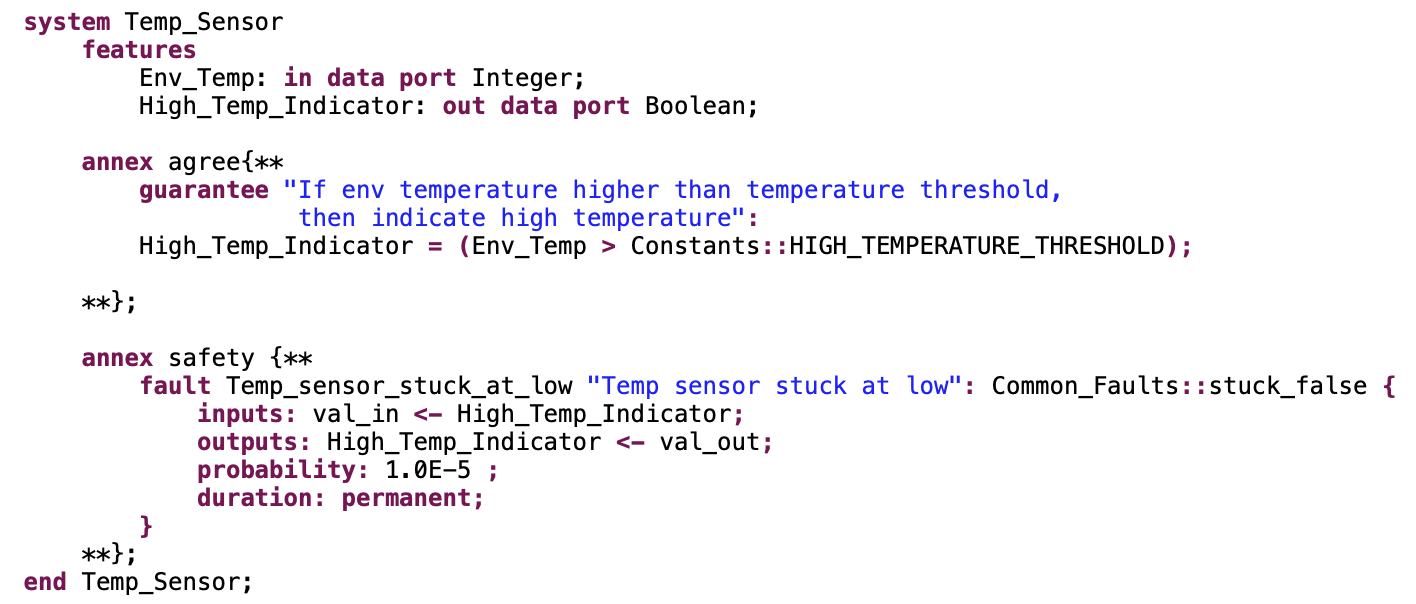
\includegraphics[width=0.9\textwidth]{images/tempSensoraadlannex.png}
	\end{center}
	%\vspace{-2em}
	\caption{Temperature sensor in AADL with AGREE and safety annexes}
	\label{fig:tempSensor}
	%\vspace{-2em}
\end{figure*}

%\textbf{Compositional Analysis} 
%One way to structure compositional verification is hierarchically: layers of the system architecture are analyzed independently and their composition demonstrates a system property of interest. Compositional verification partitions the formal analysis of a system architecture into verification tasks that correspond into the decomposition of the architecture~\cite{clarke1989compositional}.  A proof consists of demonstrating that the system property is provable given the contracts of its direct subcomponents and the system assumptions~\cite{cofer2012compositional,clarke1989compositional}. When compared to monolithic analysis (i.e., analysis of the flattened model composed of all components), the compositional approach allows the analysis to scale to much larger systems~\cite{NFM2012:CoGaMiWhLaLu,heckel1998compositional,cofer2012compositional}.

\textbf{Assume Guarantee Reasoning Environment}
The Assume Guarantee Reasoning Environment (AGREE) is a tool for formal analysis of behaviors in AADL models and supports compositional verification~\cite{cofer2012compositional}.  It is implemented as an AADL annex and is used to annotate AADL components with formal behavioral contracts. Each component's contracts includes assumptions and guarantees about the component's inputs and outputs respectively. AGREE translates an AADL model and the behavioral contracts into Lustre~\cite{Halbwachs91:IEEE} and then queries the \jkind model checker to conduct the back-end analysis~\cite{2017arXiv171201222G}. Figure~\ref{fig:tempSensor} shows the guarantee defined in the temperature sensor written in the AGREE annex.

%\textbf{JKind}
%JKind is an open-source industrial infinite-state inductive model checker for safety properties~\cite{2017arXiv171201222G}. Models and properties in JKind are specified in Lustre~\cite{Halbwachs91:IEEE}, a synchronous dataflow language, using the theories of linear real and integer arithmetic. JKind uses SMT-solvers to prove and falsify multiple properties in parallel.

\textbf{Safety Annex for AADL}
The Safety Annex for AADL provides the ability to reason about faults and faulty component behaviors in AADL models~\cite{Stewart17:IMBSA,stewart2020safety}. In the Safety Annex approach, AGREE is used to define the nominal behavior of system components, faults are introduced into the nominal model, and JKind is used to analyze the behavior of the system in the presence of faults. Faults describe deviations from the nominal behavior and are attached to the outputs of components in the system. An example of a safety annex fault definition on the temperature sensor is shown in Figure~\ref{fig:tempSensor}. The fault is associated with the \texttt{High\_Temp\_Indicator} output and has a probability of occurrence of $1.0 \times 10^{-5}$. The behavior of the output when the fault is active is to report low temperature. 
\section{Implementation}
\label{sec:impl}
%%%%%%%%%%%%%%%%%%%%%%%%%%%%%%%%%%%%%%%%%%%%%%%%%
%%%%%%%%%%%%%%%%%%%%            ALGORITHM DETAILS
%In the formalism section, we viewed the problem from the perspective of an arbitary guarantee in the model that can potentially be violated. This resulted in explicit faults at the leaf level and violated guarantees (``nondeterministic faults") at the middle/top layers. Each MCS generated at each level gives insight into the system at that level. In this section, we describe the implementation of compositional generation of minimal cut sets. %Minimal cut sets traditionally contain explicitly defined faults as elements; to this end, we implemented a compositional mapping from explicit faults to the guarantees they violate. The end result are the minimal cut sets that contribute to a violation of the top level safety property. 
In the formalism, any guarantee in the model had an associated fault activation literal and could be unconstrained. In the implementation, we rely on the fault model created in the safety annex to dictate which guarantees can be violated and how they may fail. Each explicit fault defined in the safety annex is added to the Lustre program as are assocated fault activation literals~\cite{Stewart17:IMBSA,stewart2020safety}. This corresponds to the $f_i$ and $\mathit{af}_i$ described in Section~\ref{sec:formalization}. 

\begin{figure}[h!]
	%\vspace{-2em}
	\begin{center}
		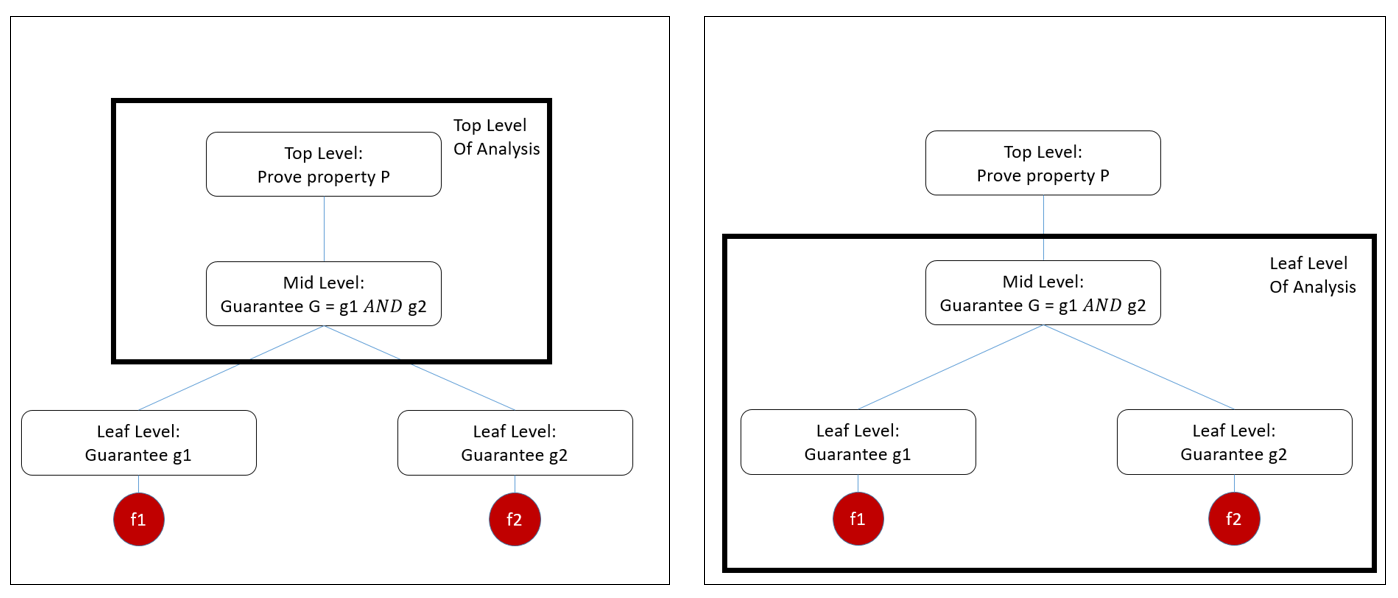
\includegraphics[width=0.9\textwidth]{images/twoLevels.PNG}
	\end{center}
	\vspace{-2em}
	\caption{Illustration of Two Layers of Analysis}
	\label{fig:layers}
\end{figure}

The \aivcalg algorithm requires that equations in the Lustre model are flagged for consideration in the analysis; these we call \emph{IVC algorithm elements}. All equations in the model can be used as IVC algorithm elements or one can specify directly the equations to consider. In this implementation, the IVC algorithm elements are added differently depending on the layer. In the leaf architectural level, fault activation literals are added to the IVC algorithm elements and are constrained to {\em false}. In middle or top layers, supporting guarantees are added. This is shown in Figure~\ref{fig:layers}. The figure shows an arbitrary architecture with two analysis layers: top and leaf. The top layer analysis adds $G$ as IVC algorithm element; the leaf layer analysis adds $f_1$ and $f_2$. 

A requirement of the hitting set algorithm is that to find all MCSs, all MUSs must be known. Ghassabani et al.~\cite{Ghassabani2017EfficientGO} showed that finding all MIVCs is as hard as model checking. It is a requirement of this analysis that all MIVCs are found. Once the MIVC analysis is complete for a property at a given layer, a hitting set algorithm is used to generate the related MCSs~\cite{murakami2013efficient}. Depending on the layer of analysis, the MCSs contain either guarantees or fault activation literals.

%For a safety property $P$, the set of all MCSs are understood as $\lor^{n}_{i=1} \mathit{MCS_i}(P)$; intuitively, this means if all constraints found in any single MCS are removed from the constraint system, $\neg P$ is satisfied. For each element $gf_j \in \mathit{MCS_i}$, this is understood as $\land^{m}_{i=1} \mathit{gf_i}$ and speaks to the minimality of the correction set. Thus the MCSs form a disjunctive normal formula over the safety property at that layer. As the proof proceeds down the hierarchy, each of the subcomponent guarantees become a property to be proven and thus MIVCs/MCSs are generated. The composition of the MCSs consists of replacing a contract in a higher layer MCS with the disjunctive normal formula of its own MCSs. After all replacements have been made, the system property formula is converted back into disjunctive normal form. 

The composition of these results is performed top down and shown in Algorithm~\ref{alg:compose}. For each guarantee found in an MCS, a replacement is made with the guarantees own MCSs. This is done recursively until all replacements have been made (line 7, 8 of Algorithm~\ref{alg:compose}). If on the other hand there are no MCSs for a given guarantee, that guarantee is replaced by its associated fault activation literal (line 10). At the leaf level of analysis, no guarantees have associated MCSs and thus reaches the end of recursion. At that time, the formula is converted back into disjunctive normal form to finish the translation into the traditional fault tree (line 11). 

\begin{algorithm}[h]
\SetKwFunction{Resolve}{resolve}
 \SetKwProg{Fn}{Function}{:}{}

	$R \gets \mathit{\amcs(P)} = \lor_{i=1}^n \mathit{MCS_i}$\\
	where $\mathit{MCS_i} = \land_{j=1}^m \mathit{gf_j}$\\
	\Fn{\Resolve{$R$}}{
		
		\For{$\forall$ OR-node in $R$}{
			\For{$\forall \mathit{gf_j}$ in OR-node}{
				\eIf{ $\exists \mathit{MCS(gf_j)}$ }{
				$R \gets$ replace $gf_j$ in $R$ with $\mathit{\amcs(gf_j)}$\;
				\Resolve($\mathit{\amcs(gf_j)}$)\;
			}{
				$R \gets $ replace $\mathit{gf_j}$ in $R$ with $\mathit{af_j}$\;	
			} 
			}
		}
		convert $R$ to DNF 
	}
	\caption{Compose Results}
	\label{alg:compose}
\end{algorithm}

Algorithm~\ref{alg:compose} provides the outline for the general case of composing fault forests: for each each property in a layer, the algorithm is called. Each property may have a corresponding fault tree. The collection of fault trees associated with each property make the forest. In the next subsection, we describe how this general algorithm is adjusted.

\begin{comment}
The number of replacements $r$ that are made for a single property $P$ are constrained by the number of minimal cut sets there are for each of the $\alpha$ contracts within the initial MCS. We call the set of all minimal cut sets for a contract $g$: $\mathit{Cut(g)}$. The following formula defines an upper bound on the number of replacements. 

\begin{lemma}
The number of replacements $r$ is bounded by the following formula:
\begin{gather}
\label{eq:bound}
  r \leq {\displaystyle \sum_{i=1}^{\alpha} }({\displaystyle \prod_{j=1}^{i} |\mathit{Cut(g_j)}|})  
\end{gather}
\begin{proof}
Assume there exists a $g_i \in \mathit{MCS(P)}$. The number of replacements made for $g_i$ is at most $|\mathit{Cut(g_i)}|$. Iteratively perform this replacement for all $\alpha$ contracts in $\mathit{MCS(P)}$. In the worst case, $|\mathit{Cut(g_1)}| \times |\mathit{Cut(g_2)}| \times \cdots \times |\mathit{Cut(g_\alpha)}|$ replacements are made.
\label{lemma:bound}
\end{proof}
\end{lemma}

\end{comment}

It is important to note that the algorithm terminates. 
\begin{theorem}
Algorithm~\ref{alg:compose} terminates
\begin{proof}
No infinite sets are generated by the \aivcalg or minimal hitting set algorithms~\cite{Ghassabani2017EfficientGO,murakami2013efficient}; therefore, for all $g_i$ in the model, $\amcs(g_i)$ is a finite set and $\mathit{MCS(g_i)}$ is a finite set.  Each call to \texttt{\small{Resolve}}\xspace processes a guarantee that was not previously resolved, and for all $g_i$ at the leaf layer of analysis, $\amcs((g_i) = \emptyset$. Given that there are finite layers in a model, the algorithm terminates.  
\end{proof}
\end{theorem}

This algorithm assumes a complete enumeration of minimal IVCs and the completion of the hitting set algorithm. These steps of analysis are not trivial to perform. We discuss these difficulties further in Section~\ref{sec:disc}.

\subsection{Pruning to Address Scalability}
Given that the growth of the DNF formula can grow quite quickly in the worst case, we implemented strategies to prune the size of the cut sets and hence the growth of these intermediate sets. The safety annex provides the capability to specify a type of verification in what is called a \textit{fault hypothesis statement}. These come in two forms: maximum number of faults or probabilistic analysis. Algorithm~\ref{alg:compose} is the general approach, but the implementation changes slightly depending on which form of analysis is being performed. This pruning improves performance and diminishes the problem of combinatorial explosion in the size of minimal cut sets for larger models. 

\textbf{Guarantees with no associated faults} If a guarantee is found in a minimal correction set and no fault has been defined in the model that can violate it, this minimal correction set (and hence the entire subtree) is pruned.

\textbf{Max \textit{n} faults analysis} The max $n$ fault hypothesis in the safety annex restricts the number of faults that can be independently active simultaneously. This statement restricts the cardinality of minimal cut sets generated to $n$. If the number of elements in an MCS exceeds the threshold of the hypothesis statement, that MCS is eliminated from consideration and its subtree is pruned.

\textbf{Probabilistic analysis pruning} A probabilistic hypothesis statement restricts the cut sets by use of a probabilistic threshold. Assuming independence between faults, any cut sets with combined probability higher than the given probabilistic threshold are removed from consideration. The allowable combinations of faults are calculated before Algorithm~\ref{alg:compose} begins; this allows for dynamic pruning of minimal correction sets. If the fault activation literals within an MCS are not a subset of any allowable combination, that MCS is pruned from the formula. 

\section{Discussion}
\label{sec:disc}
There are considerations that must be made regarding this approach. These include the enumeration of all MIVCs as well as all MHSs. We discuss these preprocessing steps and then end the discussion with some brief comments on the soundness and incompleteness of compositional reasoning. 

\subsection{Minimal Inductive Validity Core Enumeration}
Ghassabani showed that determining if an inductive validity core is minimal is as hard as model checking~\cite{ghassabani_2018, Ghassabani2017EfficientGO}. The full inductive validity core algorithm does not guarantee a minimal IVC. A separate algorithm attempts to minimize the IVCs enumerated in the full algorithm. The minimization is as hard as model checking and therefore undecidable in many settings. The implementation of the MIVC algorithm times out after a set threshold and if all MIVCs cannot be enumerated, the output of the algorithm is empty, i.e., it is an {\em offline} algorithm. 

The minimal cut sets may be enumerated via MIVCs due to the dual relationship between minimal unsatsifiable subsets (MUSs) and minimal correction sets (MCSs). The MCSs cannot be found if the unsatisfiable subsets are not minimal~\cite{liffiton2016fast}. In the case of finding minimal cut sets, if an IVC is not minimal, the hitting sets of all IVCs will not necessarily be a cut set. A simple example illustrates this concept. Assume that $\{a,b,c\}$ is an IVC and the minimal IVC contains only $\{a,b\}$. Intuitively, $a$ and $b$ are sufficient to prove some safety property. Say there are two other minimal IVCs enumerated: $\{d\}$, and $\{e\}$.  The hitting sets produced will include the set $\{c, d, e\}$. Violation of these elements will not lead to violation of the safety property, for the elements $a$ and $b$ provide a proof of the property. 

Bendik et al.~implemented an algorithm that identifies MIVCs in an {\em online} manner (i.e., one by one) and can be terminated at any time~\cite{bendik2018online}. While this algorithm performs better than the original \aivcalg algorithm developed by Ghassabani~\cite{Ghassabani2017EfficientGO}, the requirement remains that all MIVCs must be found before generating the minimal hitting sets. A possible extension to our approach is to utilize the online MIVC enumeration algorithm simply for the performance benefits. 

\subsection{Minimal Hitting Sets}
Finding inclusion-minimal hitting sets for a given collection of sets is a fundamental combinatorial problem. The problem of generating the collection of MHSs for a given set family is of interest in a wide variety of domains. The computational complexity of this problem is currently unknown; nevertheless, there is an extensive literature of algorithms to generate minimal hitting sets~\cite{gainer2017minimal}. The minimal hitting set problem is equivalent to the inclusion-minimal set cover problem. An algorithm for generating MHSs can be used to enumerate minimal set covers, a classic NP-hard problem~\cite{karp1972reducibility}. 

Murakami et al.~ proposed an algorithm used for dualizing large-scale hypergraphs~\cite{murakami2013efficient}. A hypergraph $\mathcal{F}$ is a set family defined on vertex set $V$ . The dual of $\mathcal{F}$ is the set of minimal subsets $H$ of $V$ such that $F \cap H \not = \empty$ for any $F \in \mathcal{F}$ . The computation of the dual is equivalent to the minimal hitting set problem. Finding a minimal hitting set is easy; one removes vertices one by one unless one gets an empty intersection with some hyperedges. However, finding exactly all minimal hitting sets is not easy; one must check exponentially many vertex subsets that can be minimal hitting sets. Murakami introduced a bottom-up search. They build up ``sub-MHSs" until they are hitting sets, making clever use of intermediate data structures to ensure that no redundant checks are performed~\cite{gainer2017minimal}. The algorithm incorporated into the safety annex is the MMCS algorithm~\cite{murakami2013efficient}. Let $k = ||S||$ be the sum of sizes of the sets in a set family $S$. Then MMCS runs in $\mathcal{O}(k)$ time per iteration\footnote{The authors do not give explicit bounds on the number of iterations required.}.

Given the intractability of MIVC enumeration and the challenge of the hitting set problem, being able to generate minimal cut sets without reliance on these algorithms would be beneficial. We discuss this option in Section~\ref{sec:preproc}.

\subsection{Soundness, Completeness, and Minimality}
For any proof system, soundness is the most important property--it is not possible to deduce false facts. A measure of the quality or usefulness of a proof system is obtained from an investigation into completeness--every formula can be derived using that proof system. Compositional reasoning is sound~\cite{CompTechReport}, but in general incomplete~\cite{namjoshi2010completeness}. This means that we know in nominal compositional analysis, we will not prove a false property (sound). But there may be cases in which we cannot prove a property which is true given the model (incomplete). Given the assumption for our algorithms that the nominal model proves and all MIVCs are enumerated, we know that a fault tree is still valid using this approach. 

What we cannot ensure is that the cut sets after composition are necessarily minimal. The example described in Chapter~\ref{chap:granularity} illustrates this point. Furthermore, dependencies between guarantees within the model may not be reflected in composition. We are guaranteed minimality per layer, but it is possible to lose this property upon composition. 

From safety analysts perspective, this is acceptable. This approach is not meant to supplant an analyst, but to automate certain aspects of the traditional approach to SA. The analyst is still required to understand the cut sets and how they pertain to the system as a whole. 

From a probabilistic computation perspective, this may result in an unsafe probabilistic approximation. Assuming independence, the computed probability of a cut set will be less than or equal to the computed probability of a minimal cut set. An extension to this work is to provide a meaningful over-approximation to the probabilistic computations that may be performed over a compositionally derived fault tree. 











\subsection{Hierarchical Graphical Fault Trees}
We presented a formalism that defines the composition of fault forests by extending the transition system to allow for fault activation literals. This formalism is implemented by leveraging recent research in model checking techniques. %Using the idea of minimal inductive validity cores (MIVCs), which are the minimal model elements necessary for a proof of a safety property, we are able to provide fault activation literals as model elements to the \aivcalg algorithm which provides all the MIVCs that pertain to this property. These are used to generate minimal cut sets. 

An overarching goal of this dissertation is to aid a safety analyst in the assessment process, not to replace them. Throughout this research, numerous conversations with safety analysts provided guidance.%, for instance what format would be most beneficial for the outputs of analysis or how this work could meet their needs. When discussing future work for this chapter, these conversations spring to mind. 
A common artifact used in the certification process is a fault tree. Automated generation of fault trees often produces flat trees: a single root with multiple leaves. This does not show how an error propagates through the system. It is likely that analysts will create fault trees by hand as they explore the behavior of the system in the presence of faults. The safety annex output does not include graphical fault trees, but rather the Boolean expressions that describe them. Given that the analysis is performed compositionally, a hierarchical fault tree could provide meaningful information for each layer of the system. 

%Lastly, we do not explore the composition of probabilities or computing the probability of system failure. Rather we implemented a probabilistic threshold given by the user. This is perfectly sufficient for safety analysis. Each safety property has a hazard classification and associated probability. The probabilistic hypothesis of the safety annex allows for this analysis. Nonetheless, the composition of probabilities is an area that remains to be explored. 

%In the next chapter, we describe case studies and apply these analyses to larger scale systems. We discuss timing results, analysis results, and fault modeling strategies. 